\documentclass[12pt, a4paper]{article} %possible sizes are 10,11,12
\title{Sermon Notes 2023}
\author{Kian Hwee}
%To input the current time
\usepackage[nodate, 12hr]{datetime}
\date{\small Last updated: \today, \currenttime} %leave blank if dont want date

%Packages for paper formatting, figures, hyperref, etc
\usepackage{microtype}
\usepackage{geometry} %package to adjust the margins n shit of the paper
\geometry{a4paper, margin = 2cm, top = 2cm, bottom = 2cm}
\usepackage{xcolor}
\usepackage{parskip} %package to tweak paragraph skipping
\usepackage[space]{grffile} %For file names with spaces
\usepackage{graphicx}
%\graphicspath{{./Figures/}}
\usepackage{chngcntr}
\counterwithin{figure}{section}
%\counterwithin{footnote}{section}
\usepackage{float}
\usepackage{comment} 
\usepackage{wrapfig}
\setcounter{tocdepth}{2}
%\setlength{\parskip}{0.1cm} %to set the line spacing between paragraphs. I.e,
%how compact shit should be. Also affects the list environment.
\PassOptionsToPackage{hyphens}{url}
\usepackage[hidelinks]{hyperref}
\hypersetup{
    colorlinks,
    linkcolor={blue!50!black},
    citecolor={blue!50!black},
    urlcolor={blue!80!black}
}
%For quotation marks to behave well
\usepackage{csquotes}
\MakeOuterQuote{"}

%Blind text
\usepackage[english]{babel}
\usepackage{blindtext}
\blindmathtrue

%Math packages
\usepackage{amsmath}
\usepackage{amssymb}
\numberwithin{equation}{section} %numbers equations according to sections
%\allowdisplaybreaks %equations in environment can page break
\usepackage{physics}
\usepackage{amsthm}
\theoremstyle{plain}
\newtheorem{theorem}{Theorem}[section]
\theoremstyle{remark}
\newtheorem{corollary}{Corollary}[theorem]
\theoremstyle{plain}
\newtheorem{lemma}[theorem]{Lemma}
\theoremstyle{definition}
\newtheorem{definition}{Definition}[section]
\theoremstyle{remark}
\newtheorem*{remark}{Remark}

%Alternate fonts 
% \usepackage{newtxtext,newtxmath} %this is good
\usepackage{fourier} %this is good
% \usepackage{newpxtext,newpxmath} %this is good
%The rest are...meh
% \usepackage{libertine,libertinust1math} %this is quite good
% \usepackage{fouriernc} %this is quite good
% \usepackage{mathptmx} %looks quite bad
%For new look
% \usepackage{newpxtext} \usepackage[euler-digits]{eulervm} %looks disgusting

\setcounter{secnumdepth}{0}

\begin{document}
  \maketitle
  \section*{Foreword}
    Herein contains my summary of the sermons for 2023.  These sermons notes
    are mostly typed out during the sermon as the pastor preaches.  Sometimes
    I will add in some of my own clarifications/notes/thoughts to the points
    given by the pastors, hence one can safely assume that any theological
    errors found herein are to be attributed to me, not the pastors. 
  \tableofcontents %optional
  \setcounter{figure}{0}

\section{1st October 2023: In the beginning was the Word}
\subsection*{Text: John 1:1-18}
  \begin{quote}
    [1] In the beginning was the Word, and the Word was with God, and the Word was God. [2] He was in the beginning with God. [3] All things were made through him, and without him was not any thing made that was made. [4] In him was life, and the life was the light of men. [5] The light shines in the darkness, and the darkness has not overcome it.

    [6] There was a man sent from God, whose name was John. [7] He came as a witness, to bear witness about the light, that all might believe through him. [8] He was not the light, but came to bear witness about the light.

    [9] The true light, which gives light to everyone, was coming into the world. [10] He was in the world, and the world was made through him, yet the world did not know him. [11] He came to his own, and his own people did not receive him. [12] But to all who did receive him, who believed in his name, he gave the right to become children of God, [13] who were born, not of blood nor of the will of the flesh nor of the will of man, but of God.

    [14] And the Word became flesh and dwelt among us, and we have seen his glory, glory as of the only Son from the Father, full of grace and truth. [15] (John bore witness about him, and cried out, “This was he of whom I said, ‘He who comes after me ranks before me, because he was before me.’”) [16] For from his fullness we have all received, grace upon grace. [17] For the law was given through Moses; grace and truth came through Jesus Christ. [18] No one has ever seen God; the only God, who is at the Father’s side, he has made him known.
  \end{quote}
\subsection*{Notes}
\begin{itemize}
  \item{This sermon series will be on the seven “I AM” discourses in John.}
  \item{Today’s sermon is the prologue to John. Three parts for today: mystery of the Word, the coming of the light, and the Word make flesh.}
  \item{The word “Word” is translated from the greek Logos. This word had many different meanings to the different groups of people back then. The jews would have one understanding of Logos (e.g Philo of Alexandria), the stoics would have another.}
  \item{For the jews specifically, the Logos was God’s creative power in creation. So if John stopped at “the Word was God”, it would probably be ok to the Jews, c.f Philo. I.e, since the Word is God’s creative power that creates and sustains everything, the Word is God. So, proverbs 8.}
  \item{But John went on to say “the Word was with God”, and that would have riled up the Jews, because that would contradict what they thought was monotheism. So here we have John introducing the idea of the Trinity. So here, John is preparing for later where be will introduce Jesus as the Son of God, as God’s Word. }
  \item{The next statement about Jesus being the true light that is coming into the world. This one is also quite cool, it plays on the common understanding that light is good and darkness is bad. Such as in Genesis, where God said “let there be light”.}
  \item{So far, John had not said anything too mind blowing yet. So far everything he said was metaphysical in nature, and we know how philosophers like to discuss these metaphysical things. Even if the Logos of God is another divine person apart from God, this is still metaphysical.}
  \item{The most mind-blowing part of this prologue is “the Word became flesh”. This is abit mind-blowing because the Word is a metaphysical concept, but flesh is a concrete concept. Especially in the dualistic worldview of spiritual vs physical, this statement would be offensive. And especially for the Jews, since the Logos is transcendent above space and time, so how could the Word take on flesh and be embodied, stuck in a certain space-time point> \KH{(By space-time point is meant a \textit{world line})}.}
  \item{So here, John is saying that the Word is a divine person apart from God, and the Word took on human flesh to reveal the Father to the world, to be the light that gives life to all who believes, so that to those who believe, they have the right to be the children of God. }
\end{itemize}
  \section{12th February 2023: Seven seals}
\subsection*{Text: Revelation 6:1-7, 8:1-6}
  \subsubsection*{Revelation 6:1-7}
  \begin{quote}
  [1] Now I watched when the Lamb opened one of the seven seals, and I heard
  one of the four living creatures say with a voice like thunder, “Come!” [2]
  And I looked, and behold, a white horse!  And its rider had a bow, and a
  crown was given to him, and he came out conquering, and to conquer.

  [3] When he opened the second seal, I heard the second living creature say,
  “Come!” [4] And out came another horse, bright red.  Its rider was
  permitted to take peace from the earth, so that people should slay one
  another, and he was given a great sword.

  [5] When he opened the third seal, I heard the third living creature say,
  “Come!” And I looked, and behold, a black horse!  And its rider had a pair
  of scales in his hand.  [6] And I heard what seemed to be a voice in the
  midst of the four living creatures, saying, “A quart of wheat for a
  denarius, and three quarts of barley for a denarius, and do not harm the
  oil and wine!”

  [7] When he opened the fourth seal, I heard the voice of the fourth living
  creature say, “Come!” [8] And I looked, and behold, a pale horse!  And its
  rider’s name was Death, and Hades followed him.  And they were given
  authority over a fourth of the earth, to kill with sword and with famine
  and with pestilence and by wild beasts of the earth.

  [9] When he opened the fifth seal, I saw under the altar the souls of those
  who had been slain for the word of God and for the witness they had borne.
  [10] They cried out with a loud voice, “O Sovereign Lord, holy and true,
  how long before you will judge and avenge our blood on those who dwell on
  the earth?” [11] Then they were each given a white robe and told to rest a
  little longer, until the number of their fellow servants and their brothers
  should be complete, who were to be killed as they themselves had been.

  [12] When he opened the sixth seal, I looked, and behold, there was a great
  earthquake, and the sun became black as sackcloth, the full moon became
  like blood, [13] and the stars of the sky fell to the earth as the fig tree
  sheds its winter fruit when shaken by a gale.  [14] The sky vanished like a
  scroll that is being rolled up, and every mountain and island was removed
  from its place.  [15] Then the kings of the earth and the great ones and
  the generals and the rich and the powerful, and everyone, slave and free,
  hid themselves in the caves and among the rocks of the mountains, [16]
  calling to the mountains and rocks, “Fall on us and hide us from the face
  of him who is seated on the throne, and from the wrath of the Lamb, [17]
  for the great day of their wrath has come, and who can stand?”

  \subsubsection*{Revelation 8:1-6}
  [1] When the Lamb opened the seventh seal, there was silence in heaven for
  about half an hour.  [2] Then I saw the seven angels who stand before God,
  and seven trumpets were given to them.  [3] And another angel came and
  stood at the altar with a golden censer, and he was given much incense to
  offer with the prayers of all the saints on the golden altar before the
  throne, [4] and the smoke of the incense, with the prayers of the saints,
  rose before God from the hand of the angel.  [5] Then the angel took the
  censer and filled it with fire from the altar and threw it on the earth,
  and there were peals of thunder, rumblings, flashes of lightning, and an
  earthquake.

  [6] Now the seven angels who had the seven trumpets prepared to blow them.
  \end{quote}
\subsection*{Notes}
\begin{itemize}
  \item{A quick question that might arise after this passage: what is going
  on?  Why is there so much destruction?  To answer this, we must first go
  back to chapter 5.  In chapter 5 and 6, we see that nobody was worthy to
  open the scroll, except the Lamb that was slain.  When initially John saw
  that nobody could open the scroll, he wept.  He wept because that scroll
  was very important; if nobody could open the scroll, then God's plan on
  earth cannot be fulfilled.  And God's plan is to bring in His Kingdom on
  the earth.  }
  \item{Three points for today: what are God's priorities in implementing His
  plan?  What is the process by which the plan is to be implemented?  And who
  are the participants in bringing in God's plan?}
  \item{First point: what are God's priorities?  John was taken up to heaven
  to see what is to come.  But before God showed John what is to come, John
  had to see the glorious vision of God in chapter 4 and 5.  From there, we
  see that one of God's priority is to be known as the only one true God, and
  to consequently to eliminate idolatry on earth.  Another of God's priority
  is to be known as the one Lord.  When we worship the one true God, not only
  do we say that God is the creator, we say that God is the one Lord over
  all.  This is depicted by the throne of God in the centre.  What are the
  priorities of the Lamb?  First of all, the Lamb's priority is to save us
  from idolatry.  To summarise, when God brings in His plan, His priorities
  is to be known as one creator God, one Lord, and through the Lamb, one
  saviour.}
  \item{The next point: what is the process?  Clearly, there are still
  idolators on earth and there will still be idolators on earth.  Hence,
  part of the process of bringing in His plan includes judgment.  We see that
  in these seven seals, we can split the judgment into two parts; God's
  passive judgement in seals 1-4, and God's active judgement in seals 5-7.
  Passive judgment refers to God giving people up to the consequences of
  their sins and to their subsequent hardness of hearts.  This is best
  explained in Romans 1, ``God gave them up to their passions...''.
  Theologically, it is God withholding His restraining grace on sinners and
  letting sinners do what they like.  }
  \item{For example, the first seal depicts how people would give in to their
  innate desire to conquer and for authority.  The second seal depicts how
  people would die because of this warfare that is a consequence of people's
  desire to conquer.  The third seal depicts how there would be
  hyper-inflation.  A denarius is a labourer's daily wage, and ordinarily,
  that would be able for him to feed his family.  However, after the third
  seal, there would be famine due to the war and now, a labourer can only
  afford a quart of wheat.  From ancient calculations (c.f Heroditus), we
  know that a quart of wheat is enough only to feed one single person.  I.e,
  a labourer can no longer feed his family, but only himself!  Barley is
  cheaper, and hence the labourer can buy three quarts.  The fourth seal
  depicts how there would be much death due to the first three seals.}
  \item{The sixth seal depicts God's active judgement.  This where God
  directly intervenes to actively judge sinners.  And this is depicted as
  something very fierce.}
  \item{Hence, we see that judgment is part of God's process for bringing in
  His kingdom.  In today's world, we don't like to talk about God as judge.
  Yet we as a society know that we need judges (and hence we have a
  judiciary).  And yet we as a society balk when there is injustice, for
  example when a criminal gets away due to a loophole in our human justice
  system etc.  So in a sense, we as humans all crave for some sort of final
  justice so that those who got away from the human justice system will
  eventually be held accountable.  So why do people hate the idea of God as
  judge despite them all wanting just judgement?  This is because they don't
  like what God is judging.  People all want to think that they are righteous
  and beyond judgment, and they don't like the idea that they too are so bad
  as to warrant God's judgment!  This is why we need the gospel of the Lord
  Jesus to convict the world of sin.}
  \item{The last point: the participants.  Here, we look at seals $5$ and
  $7$.  Seal $5$ tells us why God has to judge the world.  Not only do the
  people of the world want to be king and rulers and hence unleash a chain of
  bad consequences on the world, they also want to persecute the remnant who
  actually speak out for justice.  The remnant are here are those who are
  faithful in their witness to God's word.  Here, we see that while God gives
  the world up to their sinful passions through His act of passive judgement,
  He also leaves a remnant on earth to speak His truth.  So in this sense, we
  are the participants of God's judgment in the sense that we participate by
  witnessing to God's Word and His justice, even if we might lose our lives
  in the process.  Also, seal $5$ also shows us that God has His own
  timeline.  While sometimes we want God to act immediately to redress our
  injustice, we must realise that God has His own timeline.}
  \item{Seal $7$ is interesting because it is quite anti-climatic.  Seal $6$
  leads to so much crying and groaning from the peoples of the earth, yet
  seal $7$ leads to silence.  If we look at the sequel, we see that after the
  seventh seal, there are seven trumpets and seven bowls.  So we must think
  of the seven trumpets and the seven bowls as part of the seventh seal.  The
  silence in a sense, is meant for the angels to prepare (see chapter 8 verse
  6) and for prayers.  In chapter 8 verse 3, we see the angel taking the
  incense which represents the prayers of the saints.  And when the angel
  pours the prayers of the saints on the earth, we see ``peals of thunder,
  rumblings, flashes of lightning, and an earthquake''.  These are the same
  things that appear after the end of the trumpet series, and after the end
  of the bowl series. }
  \item{God did not just save us, He co-opted us as workers in His harvest
  field.  When God brings in His kingdom, He could have done it alone, but He
  chose to do it through us.  The seventh seal reminds of this; God's kingdom
  will come, God's righteous judgment will come to right the world, through
  the prayers of the saints.  The prayers of the saints comes as the climax
  of the seal series, which reminds us how important our prayers are.  It is
  God's desire that in our prayer, we resonate with God's heartbeat.  In our
  prayer, our will should be conformed to God's will, so that we want to will
  the same thing God wills.  }
  \item{We participate in God's process of bringing in the Kingdom through
  our prayers for God's righteousness to be revealed and for His justice to
  be done.  God is pleased to work through our prayers.  We participate in
  God's process of bringing in the Kingdom through our witnessing for God's
  Word and perhaps losing our lives in the process.  Witnessing for God's
  Word mean putting God's priorities as our priorities.  The fact that God
  uses our work and prayers in His process of bringing in His kingdom is a
  good reminder for us that our work for Him is not futile, and in fact is
  very important.  So we can take heart and be courageous, joyful and willing
  witnesses for God.}
  \item{After the sixth seal, we see the kings of the earth trying to flee
  from God.  That is futile, as we can see from Psalm 139.  What they should
  have done instead is to flee to God.  It is counter-intuitive, but it is
  true.}
\end{itemize}
  \setcounter{figure}{0}

\section{17th September 2023: Isn't she beautiful?}
\subsection*{Text: Song of Solomon 6:4-7:10}
  \begin{quote}
    He

    [4] You are beautiful as Tirzah, my love,
        lovely as Jerusalem,
        awesome as an army with banners.
    [5] Turn away your eyes from me,
        for they overwhelm me—
    Your hair is like a flock of goats
        leaping down the slopes of Gilead.
    [6] Your teeth are like a flock of ewes
        that have come up from the washing;
    all of them bear twins;
        not one among them has lost its young.
    [7] Your cheeks are like halves of a pomegranate
        behind your veil.
    [8] There are sixty queens and eighty concubines,
        and virgins without number.
    [9] My dove, my perfect one, is the only one,
        the only one of her mother,
        pure to her who bore her.
    The young women saw her and called her blessed;
        the queens and concubines also, and they praised her.


    [10] “Who is this who looks down like the dawn,
        beautiful as the moon, bright as the sun,
        awesome as an army with banners?”


    She

    [11] I went down to the nut orchard
        to look at the blossoms of the valley,
    to see whether the vines had budded,
        whether the pomegranates were in bloom.
    [12] Before I was aware, my desire set me
        among the chariots of my kinsman, a prince.


    Others

    [13] Return, return, O Shulammite,
        return, return, that we may look upon you.


    He

    Why should you look upon the Shulammite,
        as upon a dance before two armies?


    [1] How beautiful are your feet in sandals,
        O noble daughter!
    Your rounded thighs are like jewels,
        the work of a master hand.
    [2] Your navel is a rounded bowl
        that never lacks mixed wine.
    Your belly is a heap of wheat,
        encircled with lilies.
    [3] Your two breasts are like two fawns,
        twins of a gazelle.
    [4] Your neck is like an ivory tower.
    Your eyes are pools in Heshbon,
        by the gate of Bath-rabbim.
    Your nose is like a tower of Lebanon,
        which looks toward Damascus.
    [5] Your head crowns you like Carmel,
        and your flowing locks are like purple;
        a king is held captive in the tresses.


    [6] How beautiful and pleasant you are,
        O loved one, with all your delights!
    [7] Your stature is like a palm tree,
        and your breasts are like its clusters.
    [8] I say I will climb the palm tree
        and lay hold of its fruit.
    Oh may your breasts be like clusters of the vine,
        and the scent of your breath like apples,
    [9] and your mouth like the best wine.


    She

    It goes down smoothly for my beloved,
        gliding over lips and teeth.


    [10] I am my beloved’s,
        and his desire is for me.
  \end{quote}
\subsection*{Notes}
\begin{itemize}
  \item{To think: why do couples treat each other differently before and after marriage?}
  \item{Marriage is not the end of a r/s, it is the start of a lifelong pursuit.}
  \item{In today’s text, the man is always telling the woman how beautiful she is. He has been doing this since their courtship says, and he did this during the wedding, and he is doing it now after marriage again. He is also doing it after a fight (c.f 6:4, 7:1,6).}
  \item{Btw, today’s text is q similar to chapter 4:1-3, very similar metaphors are used.}
  \item{Seems like today’s text show that the man and woman have reconciled after their fight (see ch6:12, ch7:10). No doubt these words of love were helpful; they show the other person that regardless of how bad the fight is, the affection that y’all have for each other is unchanged, and hence they provide the security for the other person to be vulnerable. }
  \item{And ofc, the same principle holds for other interpersonal r/s too (maybe without the erotic component). In our friendships/dealing with our families, we must still love the other person and demonstrate our love even in the midst of a conflict. This demonstration would look like a desire for reconciliation, a seeking for the other person’s forgiveness, a seeking to make restitution for the wrong inflicted, etc. And when we do so, the other person will feel safe to be vulnerable with us and let us know how exactly we hurt them, and then when we address the hurt, this would lead to a growth in closeness and finally reconciliation.}
  \item{In our text, in v4, tirzah and jerusalem are the two capital cities of israel and judah back then. And then there’s also the phrase “awesome as an army with banners”. The same phrase appears in v10, that’s how we know its an inclusio. The whole chunk here then is a description of the wife’s beauty. In this section, the focus is on the wife’s face.}
  \item{The next chunk here in the description of the woman’s beauty is in ch6:13-7:5. The description here starts from bottom up. Some metaphors to take note: damascus is the capital city of the syrians, which are israel’s enemies. Hence the woman’s nose pointing towards damascus signifies an unfearing and brave spirit (much like what is praised in 1 peter 3:1-7). }
  \item{The tl;dr is then this: the woman is beautiful.}
  \item{Here, we also see that the man here is a one-woman man (chapter 6:v9). Unlike solomon!!!!}
  \item{A note on the theology of the body:
  \begin{itemize}
    \item{Bodily beauty points to the beauty of the creator. In fact, all beauty points toward the beauty of God. All creation praises God, and they do so by radiating their beauty, through which we see the wisdom and the beauty of God. Humans best reflect God’s beauty, since is humans are made in the image of God. The image of God should point us back to God.}
    \item{Jesus’ incarnation, death and resurrection took place while He was in the body. God cares about the body! In the future, there will be a \textbf{bodily resurrection}!}
  \end{itemize}}
  \item{Application: husband and wife should continue appreciating each other, physical beauty included! And when we do this, we will see God :).}
  \item{Application 2: we also shouldn’t need to chase after an ideal body image, because that differs from culture to culture! In the past, people loved women with pudgy bodies (e.g belly like a heap of wheat). Defo not today. Each of us has been fearfully and wonderfully made by God, so we should be thankful for the physical qualities God has given us :). In fact, appreciation of physical appearance is in the eye of the beholder! Shulammite thinks she is dark, but the man loves her for it.}
  \item{Application 3: in fact when we look at the man’s description of his wife, not all his description are of the wife’s physical appearance, some of them are of the wife’s qualities. E.g, nose like the tower of lebanon that looks towards damascus-> confidence. Awesome as an army with banners -> exudes strength. }
  % \item{\begin{figure}[H]
  %   \centering
  %   % 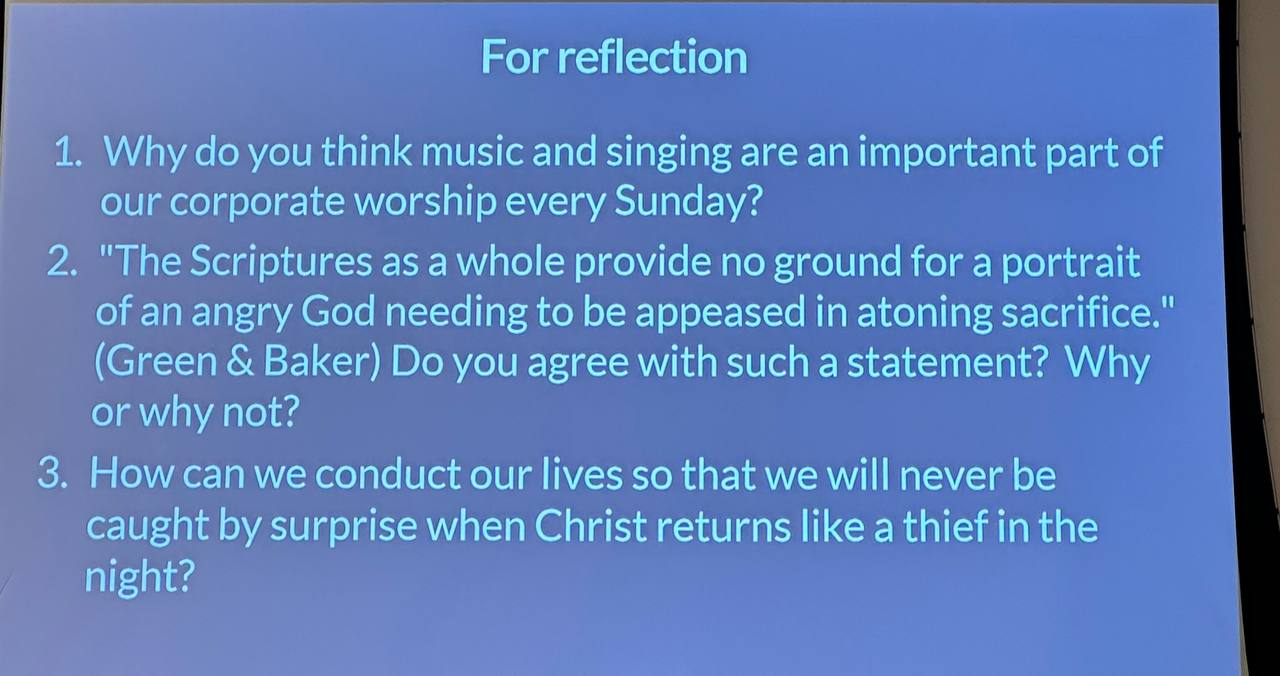
\includegraphics[width=0.8\textwidth, trim={0cm 0cm 0cm 0cm},clip]{Figures/marchSermon4Reflections.jpg}
  %   \includegraphics[width=0.8\textwidth, trim={0cm 0cm 0cm 0cm},clip]{example-image-a}
  %   \caption[]{Reflection questions for this sermon}
  %   \label{}
  % \end{figure}}
\end{itemize}
  \section{23rd October 2022: Are you a lukewarm Christian?}
\subsection*{Text: Revelation 3:14-22}
  \begin{quote}
    [14] “And to the angel of the church in Laodicea write: ‘The words of the Amen, the faithful and true witness, the beginning of God’s creation.

    [15] “‘I know your works: you are neither cold nor hot. Would that you were either cold or hot! [16] So, because you are lukewarm, and neither hot nor cold, I will spit you out of my mouth. [17] For you say, I am rich, I have prospered, and I need nothing, not realizing that you are wretched, pitiable, poor, blind, and naked. [18] I counsel you to buy from me gold refined by fire, so that you may be rich, and white garments so that you may clothe yourself and the shame of your nakedness may not be seen, and salve to anoint your eyes, so that you may see. [19] Those whom I love, I reprove and discipline, so be zealous and repent. [20] Behold, I stand at the door and knock. If anyone hears my voice and opens the door, I will come in to him and eat with him, and he with me. [21] The one who conquers, I will grant him to sit with me on my throne, as I also conquered and sat down with my Father on his throne. [22] He who has an ear, let him hear what the Spirit says to the churches.’”
  \end{quote}
\subsection*{Notes}
\begin{itemize}
  \item{What does lukewarm even mean? What is Jesus trying to say with the word ``lukewarm''? Three points:
  \begin{enumerate}
    \item{The assessor: who is the one doing the assessment?}
    \item{The assessment: what is the assessment given to the church in Laodicea?}
    \item{The advice: after the assessment, what is the advice that Jesus gives?}
  \end{enumerate}
  This is the last letter, and hence it is quite significant. In mose letters to the churches there is both commendation and rebuke. Except for Philadelphia and Smyrna, where there is only commendation. Here, to Laodicea, there is only rebuke.}
  \item{Point 1: The assessor.
  \begin{itemize}
    \item{The letter starts with Jesus telling the church his titles.  Here
    there are three titles:
    \begin{enumerate}
      \item{The Amen}
      \item{Faithful and true}
      \item{The beginning of God's creation}
    \end{enumerate}}
    \item{Amen means something sure, something firm, something valid.  So
    when we end our prayers with amen, we are saying to God “let our prayers
    be sure, be firm, be valid”.  So when Jesus calls himself the Amen, he is
    saying that he is sure, he is firm.  Steadfast.}
    \item{Next, Jesus is the faithful and true witness.  The word witness and
    amen links to truth.  So what Jesus is saying is true and hence worth
    listening to.}
    \item{Lastly, “beginning of Gods creation” refers to Jesus being the
    creator.  Jesus is the Word of the Father, eternally begotten, through
    whom all things are made.  Hence, since Jesus is the creator, what he
    says about the Laodiceans is significant because he created them.}
    \item{Jesus reminds us of these titles to prompt us to realise.
    Sometimes we know these titles but we forget their significance.  We need
    to hear them anew to learn that we must submit to Jesus’ voice.}
  \end{itemize} }
  \item{Point 2: The assessment.
  \begin{itemize}
    \item{Similar to the other letters, we also have Jesus saying “i know your works”. The church in Laodicea is lukewarm. But what does lukewarm mean? The key to understanding “lukewarm” in this text is to look at the “for” in verse 17.}
    \item{In verse 17, we see that the church in Laodicea had a particular
    assessment of themselves.  They say that they are rich, they say that
    they have prospered (so they got the wealth themselves), and lastly they
    say that they need nothing.  The last one is particularly fatal; when one
    thinks that he is self-sufficient, he thinks that he doesn’t need Jesus.
    Then he is not open to receiving from Jesus.  This is human nature 101;
    when we are full of ourselves, we won’t listen to what other people say
    and we won’t learn anything.  That is pride.  Compare with the
    beautitudes: “blessed are the poor in spirit”.}
    \item{In contrast to their self assessment, Jesus, the faithful and true, told them about their actual state. They are poor and pitiable, wretched, blind and naked.}
    \item{In those days, Laodicea was a very rich city because of their wool trade. They had some sheep that produced glossy black wool lol. Also, they were a city famous for eye doctors (ophthalmologists). The city was so rich that when they had an earthquake, they told their roman overlords that they didnt need any help. }
    \item{Here we see that Jesus' rebuke was especially relevant to the city of Laodicea; naked <-> wool trade, blind <-> eye doctor.}
    \item{So what exactly is lukewarm?  From our archeological evidence, we
    see that Laodicea was on a plateau.  They had no natural sources of
    water.  Their water was piped, and hence they had neither hot water or
    cold water (the water would equilibrate to a lukewarm steady state in the
    pipes).  And lukewarm water back then had no use (can’t make cold food
    nor hot food).  So Jesus is saying that the Laodiceans in their current
    state is of no use to him.  We see that despite the city’s riches, they
    could not solve this water problem themselves.  Similarly, despite the
    city’s supposed self-sufficiency, they cant solve their own spiritual problems.}
  \end{itemize}}
  \item{Point 3: The advice.
  \begin{itemize}
    \item{Since the Laodiceans can't solve their own spiritual problems
    themselves, they need to buy spiritual things from Jesus, like gold
    refined by fire (not like the gold they have they will decay), white
    garments (not like their earthly garments), and eye balm (not like what
    their eye doctors give).}
    \item{Last piece of advice given is that Jesus says that he is at the
    door and knocking.  He wants us to hear his voice and open the door for
    him to come in.  Why is Jesus knocking?  Because my heart's door is
    closed.  But why is my door closed?  Either because of hardness of heart,
    or because of shame.  If it is the latter, then that is silly because we
    must know that we can't deal with shame ourselves.  We need Jesus to help
    us deal with sin and shame, it is wrong to think that we need to deal
    with sin and shame first before we can open our heart to Jesus.  We are
    not self-sufficient.  We need Jesus.}
    \item{And when we open our heart to Jesus, Jesus will fellowship with us, and we will sit with Jesus in glory in the last days.}
  \end{itemize}
  }
\end{itemize}
  \section{29th January 2022: The Redeeming Lamb}
\subsection*{Text: Revelation 5}
  \begin{quote}
    [1] Then I saw in the right hand of him who was seated on the throne a scroll written within and on the back, sealed with seven seals. [2] And I saw a mighty angel proclaiming with a loud voice, “Who is worthy to open the scroll and break its seals?” [3] And no one in heaven or on earth or under the earth was able to open the scroll or to look into it, [4] and I began to weep loudly because no one was found worthy to open the scroll or to look into it. [5] And one of the elders said to me, “Weep no more; behold, the Lion of the tribe of Judah, the Root of David, has conquered, so that he can open the scroll and its seven seals.”

    [6] And between the throne and the four living creatures and among the elders I saw a Lamb standing, as though it had been slain, with seven horns and with seven eyes, which are the seven spirits of God sent out into all the earth. [7] And he went and took the scroll from the right hand of him who was seated on the throne. [8] And when he had taken the scroll, the four living creatures and the twenty-four elders fell down before the Lamb, each holding a harp, and golden bowls full of incense, which are the prayers of the saints. [9] And they sang a new song, saying,

    “Worthy are you to take the scroll
        and to open its seals,
    for you were slain, and by your blood you ransomed people for God
        from every tribe and language and people and nation,
    [10] and you have made them a kingdom and priests to our God,
        and they shall reign on the earth.”

    [11] Then I looked, and I heard around the throne and the living creatures and the elders the voice of many angels, numbering myriads of myriads and thousands of thousands, [12] saying with a loud voice,

    “Worthy is the Lamb who was slain,
    to receive power and wealth and wisdom and might
    and honor and glory and blessing!”

    [13] And I heard every creature in heaven and on earth and under the earth and in the sea, and all that is in them, saying,

    “To him who sits on the throne and to the Lamb
    be blessing and honor and glory and might forever and ever!”

    [14] And the four living creatures said, “Amen!” and the elders fell down and worshiped.
  \end{quote}
\subsection*{Notes}
\begin{itemize}
  \item{Three points for today: disappointment, solution, and response.}
  \item{Verse 4 tells us at the start, there was a scroll that was sealed
  completely (7 seals, 7 is the number of perfection).  Unfortunately,
  nothing in creation (in heaven, on earth or under the earth) could open the
  scroll.  This scroll was important because it contained God's plan of
  salvation and judgment.  If nobody could open the scroll, then the plan of
  salvation and judgment could not be carried out.  Hence, the weeping.}
  \item{We live in a world that is VUCA (volatile, uncertain, complex and
  ambiguous).  We face many disappointments in life, from people, from
  unanswered prayers, etc.  And that is because of sin and the fall of Man.
  Verse 4 tells us that creation cannot save itself.  This means that when we
  look to someone or something for hope, we can't look to someone or
  something in creation for hope.  We must look outside.}
  \item{Verses 5-9 give us the solution to the problem in v4.  An elder told
  John that $\exists$ (there exists) someone who can break the seals and open
  the scroll, and that someone was the Lion from the tribe of Judah (c.f Gen
  49:9-10), from the root of Jesse.  Obviously, this someone was the
  long-promised messiah. }
  \item{But shockingly, when John turned around, he saw a lamb instead! The expectation of the Lion of Judah that was to come was fulfilled by the Lamb of God. Lion represents an animal that is strong, and Lamb represents an animal that is meek. A few questions that comes to mind:
  \begin{enumerate}
    \item{Who is the Slain Lamb? (Jesus as the fulfilment of the passover Lamb).}
    \item{Why is He worthy to open the scroll and the seals?  ( He has made
    all of us sinners a people for God through His blood.  He has already
    triumphed over evil by taking on the world's evil on himself, dying and
    resurrecting.)}
    \item{How did He conquer?  (Not with might and strength like the rulers
    of the world, but with the sacrificial meekness of a Lamb.  This is
    mind-blowing!  This Lamb is actually very powerful, with seven horns.
    This Lamb is also all knowing, with seven eyes.  THis Lamb is very
    powerful, but He wins the victory through His sacrificial death and
    through His resurrection.)}
    \item{What does it mean for us today?  (We are redeemed to be witnesses
    of Christ, to live like Christ.  This means that for us Christians today,
    the way we win is the same way Christ wins; we win not by strength,
    military or political, but we win by self-sacrificial meekness that
    touches the hearts of others.)}
  \end{enumerate}}
  \item{Also, Christ has redeemed people from every tribe and nation and
  tongue and tribe.  This means that God, from the start, desires a
  multi-cultural body of Christ.  There is unity in diversity, rather than
  uniformity.  True worship focuses on something more important than
  ourselves, it is focused on Christ.  All races stand in need of a saviour,
  and all races have the same savior.  The savior is what unites us.}
  \item{Our savior Jesus died for our sins but He rose again, and He will
  come again to reign.  When we follow Jesus' example, we don't need to be
  afraid of dying. For like Jesus, it is through death that we overcome, and
  like Jesus, God will raise us up to reign with Jesus through His Holy Spirit.}
  \item{Verses 8-14 is the response of all creation.  They sang a new song,
  just like Psalm 98.  When we know the magnitude of what Christ has done for
  us, and when we know that Christ can do what He was done only because of
  His worthiness, we will naturally worship and celebrate.  The
  worship of the Lamb here in chapter 5 is the same as the worship of the one
  on the throne in chapter 4.  Just like how the figure on the throne in
  chapter 4 is in the middle of all things, the Lamb is also in the middle of
  all things.  Hence, Jesus, like the Father, is central to all creation.
  Hence, all creation's appropriate response to God is worship.  The ultimate
  destiny of Mankind can only either be to join the eternal worship chorus,
  or to rebel against God.  }
  \item{This vision of the throne room in chapters 4 and 5 is meant to give
  the seven churches a sight of the true spiritual realities.
  \begin{enumerate}
    \item{For churches like Smyrna and Philadelphia who are persecuted, this
    vision reminds them that Rome is not the centre of creation, but God is.
    Only God is worthy, and God has the power to destroy evil.  Hence, this
    would encourage the Christians there to continue holding on to their
    faith in the midst of suffering, because one day, their faith in God who
    is worthy will be vindicated.}
    \item{For churches like Laodicea and Sardis, this vision reminds them
    that they must repent and turn back to God, because only God is worthy.
    If not, one day, they will be destroyed when the Lamb opens the scroll.}
  \end{enumerate}}
\end{itemize}
  \setcounter{figure}{0}

\section{1st October 2023: In the beginning was the Word}
\subsection*{Text: John 1:1-18}
  \begin{quote}
    [1] In the beginning was the Word, and the Word was with God, and the Word was God. [2] He was in the beginning with God. [3] All things were made through him, and without him was not any thing made that was made. [4] In him was life, and the life was the light of men. [5] The light shines in the darkness, and the darkness has not overcome it.

    [6] There was a man sent from God, whose name was John. [7] He came as a witness, to bear witness about the light, that all might believe through him. [8] He was not the light, but came to bear witness about the light.

    [9] The true light, which gives light to everyone, was coming into the world. [10] He was in the world, and the world was made through him, yet the world did not know him. [11] He came to his own, and his own people did not receive him. [12] But to all who did receive him, who believed in his name, he gave the right to become children of God, [13] who were born, not of blood nor of the will of the flesh nor of the will of man, but of God.

    [14] And the Word became flesh and dwelt among us, and we have seen his glory, glory as of the only Son from the Father, full of grace and truth. [15] (John bore witness about him, and cried out, “This was he of whom I said, ‘He who comes after me ranks before me, because he was before me.’”) [16] For from his fullness we have all received, grace upon grace. [17] For the law was given through Moses; grace and truth came through Jesus Christ. [18] No one has ever seen God; the only God, who is at the Father’s side, he has made him known.
  \end{quote}
\subsection*{Notes}
\begin{itemize}
  \item{This sermon series will be on the seven “I AM” discourses in John.}
  \item{Today’s sermon is the prologue to John. Three parts for today: mystery of the Word, the coming of the light, and the Word make flesh.}
  \item{The word “Word” is translated from the greek Logos. This word had many different meanings to the different groups of people back then. The jews would have one understanding of Logos (e.g Philo of Alexandria), the stoics would have another.}
  \item{For the jews specifically, the Logos was God’s creative power in creation. So if John stopped at “the Word was God”, it would probably be ok to the Jews, c.f Philo. I.e, since the Word is God’s creative power that creates and sustains everything, the Word is God. So, proverbs 8.}
  \item{But John went on to say “the Word was with God”, and that would have riled up the Jews, because that would contradict what they thought was monotheism. So here we have John introducing the idea of the Trinity. So here, John is preparing for later where be will introduce Jesus as the Son of God, as God’s Word. }
  \item{The next statement about Jesus being the true light that is coming into the world. This one is also quite cool, it plays on the common understanding that light is good and darkness is bad. Such as in Genesis, where God said “let there be light”.}
  \item{So far, John had not said anything too mind blowing yet. So far everything he said was metaphysical in nature, and we know how philosophers like to discuss these metaphysical things. Even if the Logos of God is another divine person apart from God, this is still metaphysical.}
  \item{The most mind-blowing part of this prologue is “the Word became flesh”. This is abit mind-blowing because the Word is a metaphysical concept, but flesh is a concrete concept. Especially in the dualistic worldview of spiritual vs physical, this statement would be offensive. And especially for the Jews, since the Logos is transcendent above space and time, so how could the Word take on flesh and be embodied, stuck in a certain space-time point> \KH{(By space-time point is meant a \textit{world line})}.}
  \item{So here, John is saying that the Word is a divine person apart from God, and the Word took on human flesh to reveal the Father to the world, to be the light that gives life to all who believes, so that to those who believe, they have the right to be the children of God. }
\end{itemize}
  \section{12th February 2023: Seven seals}
\subsection*{Text: Revelation 6:1-7, 8:1-6}
  \subsubsection*{Revelation 6:1-7}
  \begin{quote}
  [1] Now I watched when the Lamb opened one of the seven seals, and I heard
  one of the four living creatures say with a voice like thunder, “Come!” [2]
  And I looked, and behold, a white horse!  And its rider had a bow, and a
  crown was given to him, and he came out conquering, and to conquer.

  [3] When he opened the second seal, I heard the second living creature say,
  “Come!” [4] And out came another horse, bright red.  Its rider was
  permitted to take peace from the earth, so that people should slay one
  another, and he was given a great sword.

  [5] When he opened the third seal, I heard the third living creature say,
  “Come!” And I looked, and behold, a black horse!  And its rider had a pair
  of scales in his hand.  [6] And I heard what seemed to be a voice in the
  midst of the four living creatures, saying, “A quart of wheat for a
  denarius, and three quarts of barley for a denarius, and do not harm the
  oil and wine!”

  [7] When he opened the fourth seal, I heard the voice of the fourth living
  creature say, “Come!” [8] And I looked, and behold, a pale horse!  And its
  rider’s name was Death, and Hades followed him.  And they were given
  authority over a fourth of the earth, to kill with sword and with famine
  and with pestilence and by wild beasts of the earth.

  [9] When he opened the fifth seal, I saw under the altar the souls of those
  who had been slain for the word of God and for the witness they had borne.
  [10] They cried out with a loud voice, “O Sovereign Lord, holy and true,
  how long before you will judge and avenge our blood on those who dwell on
  the earth?” [11] Then they were each given a white robe and told to rest a
  little longer, until the number of their fellow servants and their brothers
  should be complete, who were to be killed as they themselves had been.

  [12] When he opened the sixth seal, I looked, and behold, there was a great
  earthquake, and the sun became black as sackcloth, the full moon became
  like blood, [13] and the stars of the sky fell to the earth as the fig tree
  sheds its winter fruit when shaken by a gale.  [14] The sky vanished like a
  scroll that is being rolled up, and every mountain and island was removed
  from its place.  [15] Then the kings of the earth and the great ones and
  the generals and the rich and the powerful, and everyone, slave and free,
  hid themselves in the caves and among the rocks of the mountains, [16]
  calling to the mountains and rocks, “Fall on us and hide us from the face
  of him who is seated on the throne, and from the wrath of the Lamb, [17]
  for the great day of their wrath has come, and who can stand?”

  \subsubsection*{Revelation 8:1-6}
  [1] When the Lamb opened the seventh seal, there was silence in heaven for
  about half an hour.  [2] Then I saw the seven angels who stand before God,
  and seven trumpets were given to them.  [3] And another angel came and
  stood at the altar with a golden censer, and he was given much incense to
  offer with the prayers of all the saints on the golden altar before the
  throne, [4] and the smoke of the incense, with the prayers of the saints,
  rose before God from the hand of the angel.  [5] Then the angel took the
  censer and filled it with fire from the altar and threw it on the earth,
  and there were peals of thunder, rumblings, flashes of lightning, and an
  earthquake.

  [6] Now the seven angels who had the seven trumpets prepared to blow them.
  \end{quote}
\subsection*{Notes}
\begin{itemize}
  \item{A quick question that might arise after this passage: what is going
  on?  Why is there so much destruction?  To answer this, we must first go
  back to chapter 5.  In chapter 5 and 6, we see that nobody was worthy to
  open the scroll, except the Lamb that was slain.  When initially John saw
  that nobody could open the scroll, he wept.  He wept because that scroll
  was very important; if nobody could open the scroll, then God's plan on
  earth cannot be fulfilled.  And God's plan is to bring in His Kingdom on
  the earth.  }
  \item{Three points for today: what are God's priorities in implementing His
  plan?  What is the process by which the plan is to be implemented?  And who
  are the participants in bringing in God's plan?}
  \item{First point: what are God's priorities?  John was taken up to heaven
  to see what is to come.  But before God showed John what is to come, John
  had to see the glorious vision of God in chapter 4 and 5.  From there, we
  see that one of God's priority is to be known as the only one true God, and
  to consequently to eliminate idolatry on earth.  Another of God's priority
  is to be known as the one Lord.  When we worship the one true God, not only
  do we say that God is the creator, we say that God is the one Lord over
  all.  This is depicted by the throne of God in the centre.  What are the
  priorities of the Lamb?  First of all, the Lamb's priority is to save us
  from idolatry.  To summarise, when God brings in His plan, His priorities
  is to be known as one creator God, one Lord, and through the Lamb, one
  saviour.}
  \item{The next point: what is the process?  Clearly, there are still
  idolators on earth and there will still be idolators on earth.  Hence,
  part of the process of bringing in His plan includes judgment.  We see that
  in these seven seals, we can split the judgment into two parts; God's
  passive judgement in seals 1-4, and God's active judgement in seals 5-7.
  Passive judgment refers to God giving people up to the consequences of
  their sins and to their subsequent hardness of hearts.  This is best
  explained in Romans 1, ``God gave them up to their passions...''.
  Theologically, it is God withholding His restraining grace on sinners and
  letting sinners do what they like.  }
  \item{For example, the first seal depicts how people would give in to their
  innate desire to conquer and for authority.  The second seal depicts how
  people would die because of this warfare that is a consequence of people's
  desire to conquer.  The third seal depicts how there would be
  hyper-inflation.  A denarius is a labourer's daily wage, and ordinarily,
  that would be able for him to feed his family.  However, after the third
  seal, there would be famine due to the war and now, a labourer can only
  afford a quart of wheat.  From ancient calculations (c.f Heroditus), we
  know that a quart of wheat is enough only to feed one single person.  I.e,
  a labourer can no longer feed his family, but only himself!  Barley is
  cheaper, and hence the labourer can buy three quarts.  The fourth seal
  depicts how there would be much death due to the first three seals.}
  \item{The sixth seal depicts God's active judgement.  This where God
  directly intervenes to actively judge sinners.  And this is depicted as
  something very fierce.}
  \item{Hence, we see that judgment is part of God's process for bringing in
  His kingdom.  In today's world, we don't like to talk about God as judge.
  Yet we as a society know that we need judges (and hence we have a
  judiciary).  And yet we as a society balk when there is injustice, for
  example when a criminal gets away due to a loophole in our human justice
  system etc.  So in a sense, we as humans all crave for some sort of final
  justice so that those who got away from the human justice system will
  eventually be held accountable.  So why do people hate the idea of God as
  judge despite them all wanting just judgement?  This is because they don't
  like what God is judging.  People all want to think that they are righteous
  and beyond judgment, and they don't like the idea that they too are so bad
  as to warrant God's judgment!  This is why we need the gospel of the Lord
  Jesus to convict the world of sin.}
  \item{The last point: the participants.  Here, we look at seals $5$ and
  $7$.  Seal $5$ tells us why God has to judge the world.  Not only do the
  people of the world want to be king and rulers and hence unleash a chain of
  bad consequences on the world, they also want to persecute the remnant who
  actually speak out for justice.  The remnant are here are those who are
  faithful in their witness to God's word.  Here, we see that while God gives
  the world up to their sinful passions through His act of passive judgement,
  He also leaves a remnant on earth to speak His truth.  So in this sense, we
  are the participants of God's judgment in the sense that we participate by
  witnessing to God's Word and His justice, even if we might lose our lives
  in the process.  Also, seal $5$ also shows us that God has His own
  timeline.  While sometimes we want God to act immediately to redress our
  injustice, we must realise that God has His own timeline.}
  \item{Seal $7$ is interesting because it is quite anti-climatic.  Seal $6$
  leads to so much crying and groaning from the peoples of the earth, yet
  seal $7$ leads to silence.  If we look at the sequel, we see that after the
  seventh seal, there are seven trumpets and seven bowls.  So we must think
  of the seven trumpets and the seven bowls as part of the seventh seal.  The
  silence in a sense, is meant for the angels to prepare (see chapter 8 verse
  6) and for prayers.  In chapter 8 verse 3, we see the angel taking the
  incense which represents the prayers of the saints.  And when the angel
  pours the prayers of the saints on the earth, we see ``peals of thunder,
  rumblings, flashes of lightning, and an earthquake''.  These are the same
  things that appear after the end of the trumpet series, and after the end
  of the bowl series. }
  \item{God did not just save us, He co-opted us as workers in His harvest
  field.  When God brings in His kingdom, He could have done it alone, but He
  chose to do it through us.  The seventh seal reminds of this; God's kingdom
  will come, God's righteous judgment will come to right the world, through
  the prayers of the saints.  The prayers of the saints comes as the climax
  of the seal series, which reminds us how important our prayers are.  It is
  God's desire that in our prayer, we resonate with God's heartbeat.  In our
  prayer, our will should be conformed to God's will, so that we want to will
  the same thing God wills.  }
  \item{We participate in God's process of bringing in the Kingdom through
  our prayers for God's righteousness to be revealed and for His justice to
  be done.  God is pleased to work through our prayers.  We participate in
  God's process of bringing in the Kingdom through our witnessing for God's
  Word and perhaps losing our lives in the process.  Witnessing for God's
  Word mean putting God's priorities as our priorities.  The fact that God
  uses our work and prayers in His process of bringing in His kingdom is a
  good reminder for us that our work for Him is not futile, and in fact is
  very important.  So we can take heart and be courageous, joyful and willing
  witnesses for God.}
  \item{After the sixth seal, we see the kings of the earth trying to flee
  from God.  That is futile, as we can see from Psalm 139.  What they should
  have done instead is to flee to God.  It is counter-intuitive, but it is
  true.}
\end{itemize}
\end{document}


